%----------------------------------------------------------------------------------------
%	HEADER
%----------------------------------------------------------------------------------------
% !TeX spellcheck = en_US

\documentclass[12pt, a4paper, oneside]{article}

\usepackage[english]{babel} % Language hyphenation and typographical rules

\usepackage[top=3cm, left=3cm, right=2cm, bottom=2.5cm]{geometry} % Document margins
\usepackage[hang, small,labelfont=bf,up,textfont=it,up]{caption} % Custom captions under/above floats in tables or figures
\usepackage{booktabs} % Horizontal rules in tables

\usepackage{lettrine} % The lettrine is the first enlarged letter at the beginning of the text

\usepackage{enumitem} % Customized lists
\setlist[itemize]{noitemsep} % Make itemize lists more compact

% TODO do we need a abstract?
\usepackage{abstract} % Allows abstract customization
\renewcommand{\abstractnamefont}{\normalfont\bfseries} % Set the "Abstract" text to bold
\renewcommand{\abstracttextfont}{\normalfont\small\itshape} % Set the abstract itself to small italic text

\usepackage{titlesec} % Allows customization of titles
%\renewcommand\thesection{\Roman{section}} % Roman numerals for the sections
\titleformat{\section}[block]{\large\scshape\centering}{\thesection.}{1em}{} % Change the look of the section titles
\titleformat{\subsection}[block]{\large}{\thesubsection.}{1em}{} % Change the look of the section titles

\usepackage{fancyhdr} % Headers and footers
\pagestyle{fancy} % All pages have headers and footers
\fancyhead{} % Blank out the default header
\fancyfoot{} % Blank out the default footer
\fancyhead[C]{Water Management $\bullet$ Seminar Computational Economics $\bullet$ Winter Semester 2019/2020} % Custom header text
\fancyfoot[RO,LE]{\thepage} % Custom footer text

\setlength{\parindent}{0em}

\usepackage{titling} % Customizing the title section

\usepackage{hyperref} % For hyperlinks in the PDF

\usepackage{graphicx} % for figures

\usepackage{longtable}

% packages used for citations
\usepackage[
backend=bibtex,
style=alphabetic,
citestyle=authoryear,
natbib=true
]{biblatex}
\addbibresource{collection.bib}

% TODO delete the lorem ipsum
\usepackage{blindtext} % Package to generate dummy text throughout this template 

\title{Water Management}
%----------------------------------------------------------------------------------------

\begin{document}
	
	%----------------------------------------------------------------------------------------
	%	COVER SHEET
	%----------------------------------------------------------------------------------------
	
	\begin{titlepage}
		\begin{center}
			\vspace*{1cm}
			
			\textbf{Seminar \textit{Computational Economics}}                
			
			\vspace{0.5cm}
			{\makeatletter{\@title}\makeatother}
			
			\vspace{1.5cm}
			
			\textbf{Felix Fink} \\
			stud. 2nd semester M.Sc. Business Administration and Engineering: Mechanical Engineering \\
			Matr. Nr. 345971 \\
			\href{mailto:felix.fink@rwth-aachen.de}{felix.fink@rwth-aachen.de} 
			
			\vspace{1cm}
			
			\textbf{Niklas Sayer} \\
			stud. 2nd semester M.Sc. Business Administration and Engineering: Materials- and Process Engineering\\
			Matr. Nr. 332404
			\href{mailto:niklas.sayer@rwth-aachen.de}{niklas.sayer@rwth-aachen.de} 
			
			\vspace{1cm}
			
			\textbf{Martin Wicke} \\
			stud. M.Sc. Business Administration and Engineering: Electrical Power Engineering\\
			Matr. Nr. 336301 \\
			\href{mailto:martin.wicke@rwth-aachen.de}{martin.wicke@rwth-aachen.de} 
			
			\vfill
			
			
			Supervisor\\
			Thomas Gehrmann, M.Sc.
			
			\vspace{0.8cm}
			
			%\includegraphics[width=0.4\textwidth]{university}
			
			Computational Economics\\
			RWTH Aachen University\\
			Winter Semester 2019/2020
			
		\end{center}
	\end{titlepage}

	%----------------------------------------------------------------------------------------
	%	TABLE OF CONTENTS
	%----------------------------------------------------------------------------------------
	
	\tableofcontents
	\clearpage
	
	%----------------------------------------------------------------------------------------
	%	ARTICLE CONTENTS
	%----------------------------------------------------------------------------------------
	
	\section{Introduction}
	
	\subsection{Motivation}
With world population expected to hit 9.7 billion in 2050 and 11.2 billion in 2100, more and more people have to be fed, which will increase the demand of water for agriculture uses \citep{un2019}.
Already today, around one third of the world's population live under physical water scarcity \citep{vorosmarty2000global, alcamo2003global, oki2006global}.
With climate change proceeding, rainfall as the natural influx of lakes will become more volatile in some regions while prolonged dry periods will make water an even more precious resource in other areas \citep{guhathakurta2011impact}.
This situation will get even worse due to the projected increase in the demand of water per capita in many regions of the world, driven by lifestyle factors, especially diet \citep{vorosmarty2000global}.
Despite all those challenges, research suggests that just by using water more efficiently, we will be able to meet the acute water, environment and poverty challenges facing us over the next 50 years \citep{molden2013water}.
Therefore, the optimal allocation and sustainable use of the available water will be of increasing importance in the future.


\subsection{Assumptions and Conditions}

In this work we want to examine the variations in use of water from a (hypothetical) water reservoir.
One of the most important uses of surface water is the irrigation of fields for food production. However, as farming and food production are private enterprises and lakes are public goods, interests of all different parties have to be considered.
The water reservoir to be considered has two stakeholders: farmers, who want to use the water for irrigation purposes and citizens, who want to use the lake for recreational activities.
At the beginning of every year we have to decide how much of the water from the reservoir is used for the irrigation of fields, which benefits the farmers' harvest.\\\\
The farmers utility function follows the form 

\begin{equation}
	F(x) = \frac{a_1}{1+b_1} * x^{1+b_1}
\end{equation}

where $x$ represents the amount of water to be used for irrigation in a year. The preference parameters are $a_1 = 1$ and $b_1 = -2$.\\\\

During the summer months, citizens benefit from the remaining water due to recreational use (e.g. swimming). This can be described by the recreational users' utility function which is

\begin{equation}
  G(s, x) = \frac{a_2}{1+b_2} * (s-x)^{1+b_2}
\end{equation}

with the additional paramter $s$ that indicates the water level at the beginning of the year.
For recreational users, the preference parameters shell be $a_2 = 2$ and $b_2 = -3$.\\\\

At the end of the year, water in the reservoir is replenished by rainfall, which we can assume to be randomly following a lognormal distribution \citep{oosterbaan1994frequency}:
\begin{equation}
	r \sim lognormal(\mu, \sigma^2)
\end{equation}

with parameters $\mu = 0$ and $\sigma^2 = 1$.\\\\

Other parameters are the maximum capacity of the reservoir
\begin{equation}
	M = 7
\end{equation}

and the discount factor for future utility 

\begin{equation}
	\beta = 0.9
\end{equation}

Using dynamic programming in combination with a stochastic simulation of the rainfall, we determined the optimal irrigation policy that maximizes the combined utility of farmers and citizens for a number of years $T$. 
The sequence of events for every period is displayed in figure x. 

\subsubsection{Modification 1: Variation of the discount factor}


An theoretical explanation of the used concepts will be given in chapter x

	%------------------------------------------------
	
	\section{Main Part}
	\subsection{bla}
	\begin{figure}[ht] % TODO remove example
		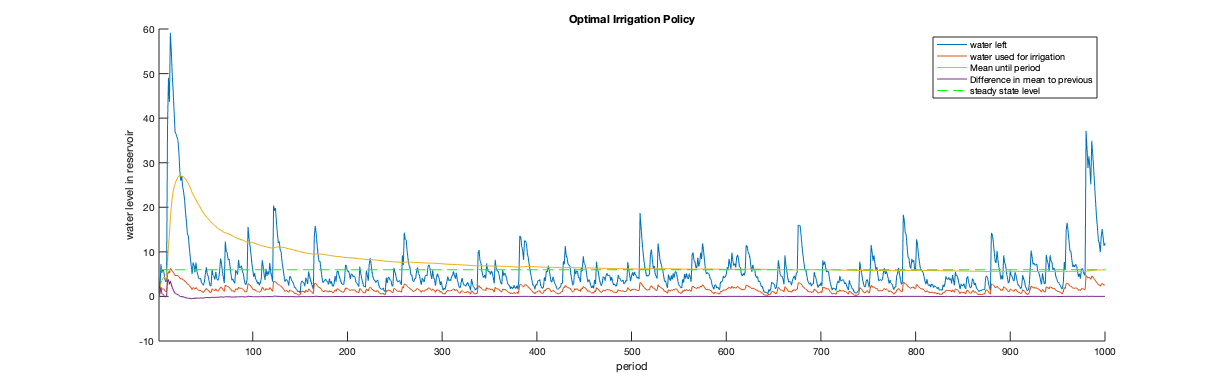
\includegraphics[width=1\textwidth]{figures/example.png}
		\caption{Example Image}
		\label{fig:example-pic}
	\end{figure}
	\blindtext
	\begin{figure}[ht] % TODO remove example
		\begin{longtable}{|p{2,5cm}|p{2,5cm}|p{2,5cm}|p{3cm}|p{3cm}|}
			\hline
			&\multicolumn{4}{c|}{\textbf{Klasse}} \\
			\hline
			& \textbf{S0} & \textbf{S1} & \textbf{S2} & \textbf{S3} \\
			\hline
			\textbf{lorem} & ipsum & ipsum & ipsum & ipsum \\
			\hline
		\end{longtable}
		\label{fig:example-figure}
		\caption{Example Table}
	\end{figure}
	\blindtext
	\blindtext
	\blindtext
	
	%------------------------------------------------
	
	\section{Conclusion}
	\blindtext

	\printbibliography

	\newpage
	
	
	%----------------------------------------------------------------------------------------
	%	STATUTORY DECLARATION IN LIEU OF AN OATH
	%----------------------------------------------------------------------------------------
	
	\begingroup
	\begin{center}
		\large
		\textbf{Eidesstattliche Versicherung}
	\end{center}
	
	\vspace{0.3cm}
	
	\begin{tabular}{@{}p{8cm}p{5.8cm}}
		\underline{\hspace{6cm}} & \underline{\hspace{5.8cm}} \\
		\vspace{0.02cm}Name, Vorname & \vspace{0.02cm}Matrikelnummer \\
	\end{tabular}
	\vspace{0.3cm}
	
	Ich versichere hiermit an Eides Statt, dass ich die vorliegende Arbeit mit dem Titel

	\begin{center}
		{\makeatletter{\emph{{\@title}}}\makeatother}
	\end{center}
	
	selbständig und ohne unzulässige fremde Hilfe erbracht habe. Ich habe keine anderen als die angegebenen Quellen und Hilfsmittel benutzt. Für den Fall, dass die Arbeit zusätzlich auf einem Datenträger eingereicht wird, erkläre ich, dass die schriftliche und die elektronische Form vollständig übereinstimmen. Die Arbeit hat in gleicher oder ähnlicher Form noch keiner Prüfungsbehörde vorgelegen.
	
	\vspace{0.6cm}
	
	\begin{tabular}{@{}p{8cm}p{5.8cm}}
		\underline{\smash{Aachen, den \today}} & \underline{\hspace{5.8cm}}\\
		Ort, Datum & Unterschrift \\
	\end{tabular}
	
	\vspace{0.6cm}

	\begin{small}
		\textbf{Belehrung:}\\
		Wer vorsätzlich gegen eine die Täuschung über Prüfungsleistungen betreffende Regelung einer Hochschulprüfungsordnung verstößt, handelt ordnungswidrig. Die Ordnungswidrigkeit kann mit einer Geldbuße bis zu 50 000 Euro geahndet werden. Zuständige Verwaltungsbehörde für die Verfolgung und Ahndung von Ordnungswidrigkeiten ist die Kanzlerin oder der Kanzler der RWTH Aachen. Im Falle eines mehrfachen oder sonstigen schwerwiegenden Täuschungsversuches kann der Prüfling zudem exmatrikuliert werden (§ 63 Abs. 5 HG NRW).
		
		\textbf{§ 156 StGB: Falsche Versicherung an Eides Statt}\\
		Wer vor einer zur Abnahme einer Versicherung an Eides Statt zuständigen Behörde eine solche Versicherung falsch abgibt oder unter Berufung auf eine solche Versicherung falsch aussagt, wird mit Freiheitsstrafe bis zu drei Jahren oder mit Geldstrafe bestraft.
		
		\textbf{§ 161 StGB: Fahrlässiger Falscheid; fahrlässige falsche Versicherung an Eides Statt}\\
		(1) Wenn eine der in den §§ 154 bis 156 bezeichneten Handlungen aus Fahrlässigkeit begangen worden ist, so tritt Freiheitsstrafe bis zu einem Jahr oder Geldstrafe ein.\\
		(2) Straflosigkeit tritt ein, wenn der Täter die falsche Angabe rechtzeitig berichtigt. Die Vorschriften des § 158 Abs. 2 und 3 gelten entsprechend
	\end{small}

	\vspace{0.6cm}
	
	Die vorstehende Belehrung habe ich zur Kenntnis genommen:
	
	\vspace{0.6cm}
	
	\begin{tabular}{@{}p{8cm}p{5.8cm}}
		\underline{\smash{Aachen, den \today}} & \underline{\hspace{5.8cm}}\\
		Ort, Datum & Unterschrift \\
	\end{tabular}
	
	\endgroup
	\clearpage
	
\end{document}
